\chapter{Rôle du préfixe cyclique dans le signal OFDM}

\section{Principe du préfixe cyclique}

Avant de répondre à cette question, nous détaillerons ici le principe d'un
préfixe cyclique et nous expliciterons sa construction. Il est à noter dans un
premier temps qu'un préfixe cyclique est un intervalle de garde
particulier\footnote{il existe deux types d'intervalle de garde: par ajout d'un
  signal nul ou par préfixe cyclique.}.


\section{Rôle du préfixe cyclique}

\subsection{Interférence inter-symboles (ISI)}


\definition{Interférence inter-symboles}{\og En télécommunications, une
  interférence inter-symbole est une forme de distorsion d'un signal qui a pour
  effet que le symbole transmis auparavant affecte le symbole aujourd'hui
  reçu\fg{}\cite{def}}


Le préfixe cyclique étant un intervalle de garde permet de se prémunir des
interférences entre symboles (ISI).

Les symboles que nous envoyons subissent des échos. Les échos correspondent aux
signal initialement envoyé mais atténué et retardé. Ils se superposent au signal
reçut de tel façon qu'a un instant $t$ il est possible de recevoir à la foi par le
signal principal le symbole $Si$ et par l'écho le symbole $S_{i-1}$: c'est l'ISI.

Si on suppose connu le temps $T_{max}$ maximal d'un écho (en pratique il est possible de
déterminer les propriétés du canal), et qu'on émet un intervalle de garde
pendant un temps $\Delta > T_{max}$ alors on recevra entre $\Delta$ et
$T_s+\Delta$ uniquement le symbole $S_i$ et l'intervalle de garde qui est
connue. Une illustration est présenté à la figure \ref{fig:intervalleGarde}.
~\\

Il n'y a donc plus d'ISI, on est capable d'extraire facilement l'information.


\begin{figure}[!h]
  \centering
  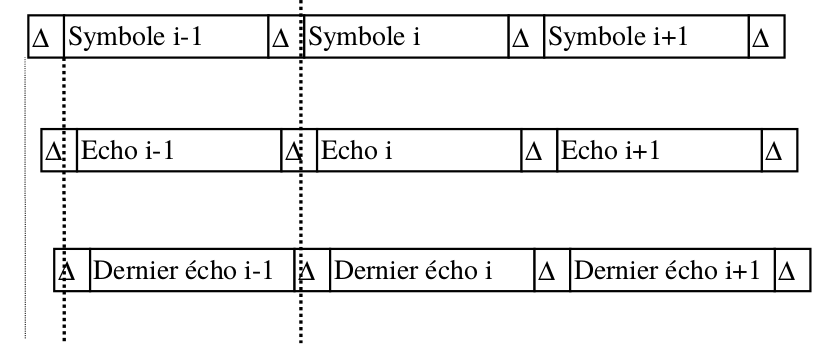
\includegraphics[width=\textwidth]{IntervalleGarde}
  \caption{Intervalle de Garde}
  \label{fig:intervalleGarde}
\end{figure}

\subsection{Interférence entre porteuses (ICI)}

\definition{Interférence entre porteuses}{Interférence dut au recouvrement des
  sous-porteuse en OFDM}

Dans ce cas ci c'est bien le caractère cyclique du préfixe qui permet d'éliminer
l'interférence entre porteuses (ICI).



%%% Local Variables:
%%% mode: latex
%%% TeX-master: "../rapport_de_base"
%%% End:
